\documentclass{beamer}
\setbeamertemplate{navigation symbols}{}

% there's no great way to make these "print-able"
%\usetheme{Madrid} not very printer-friendly
%\usecolortheme{beaver}
%\geometry{letterpaper,landscape}

% packages
\usepackage{graphicx}

% metadata
\title{Portfolio}
\author{Vaughn Kottler}
\date{\today}

\begin{document}

% slide
\begin{frame}
\frametitle{Badgerloop II: Dashboard}
    Console left (showing boot post and \texttt{help} command), data table right
\begin{center}
    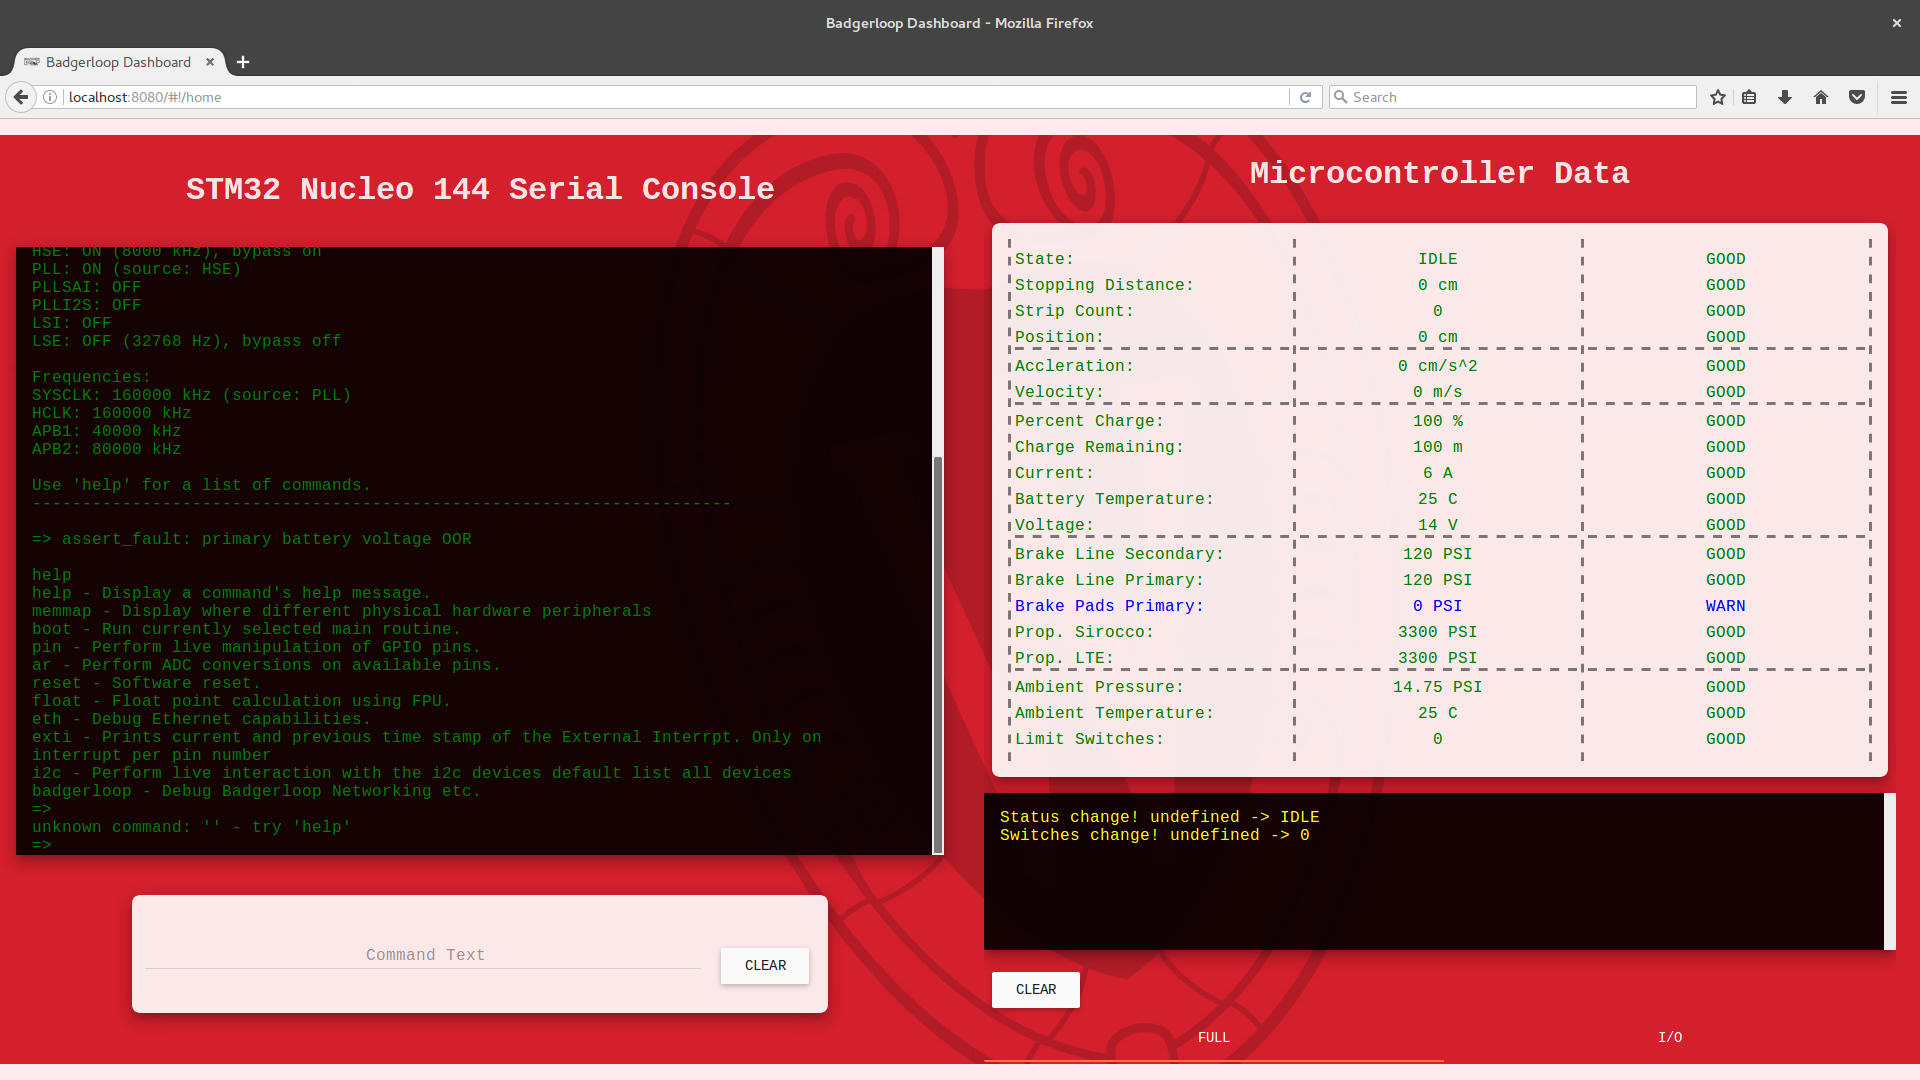
\includegraphics[width=\linewidth]{assets/badgerloop_2/Dashboard/dash_live1}
\end{center}
\end{frame}

% slide
\begin{frame}
\frametitle{Badgerloop II: Dashboard}
    Console left (showing post and \texttt{help} command), manual IO menu right
\begin{center}
    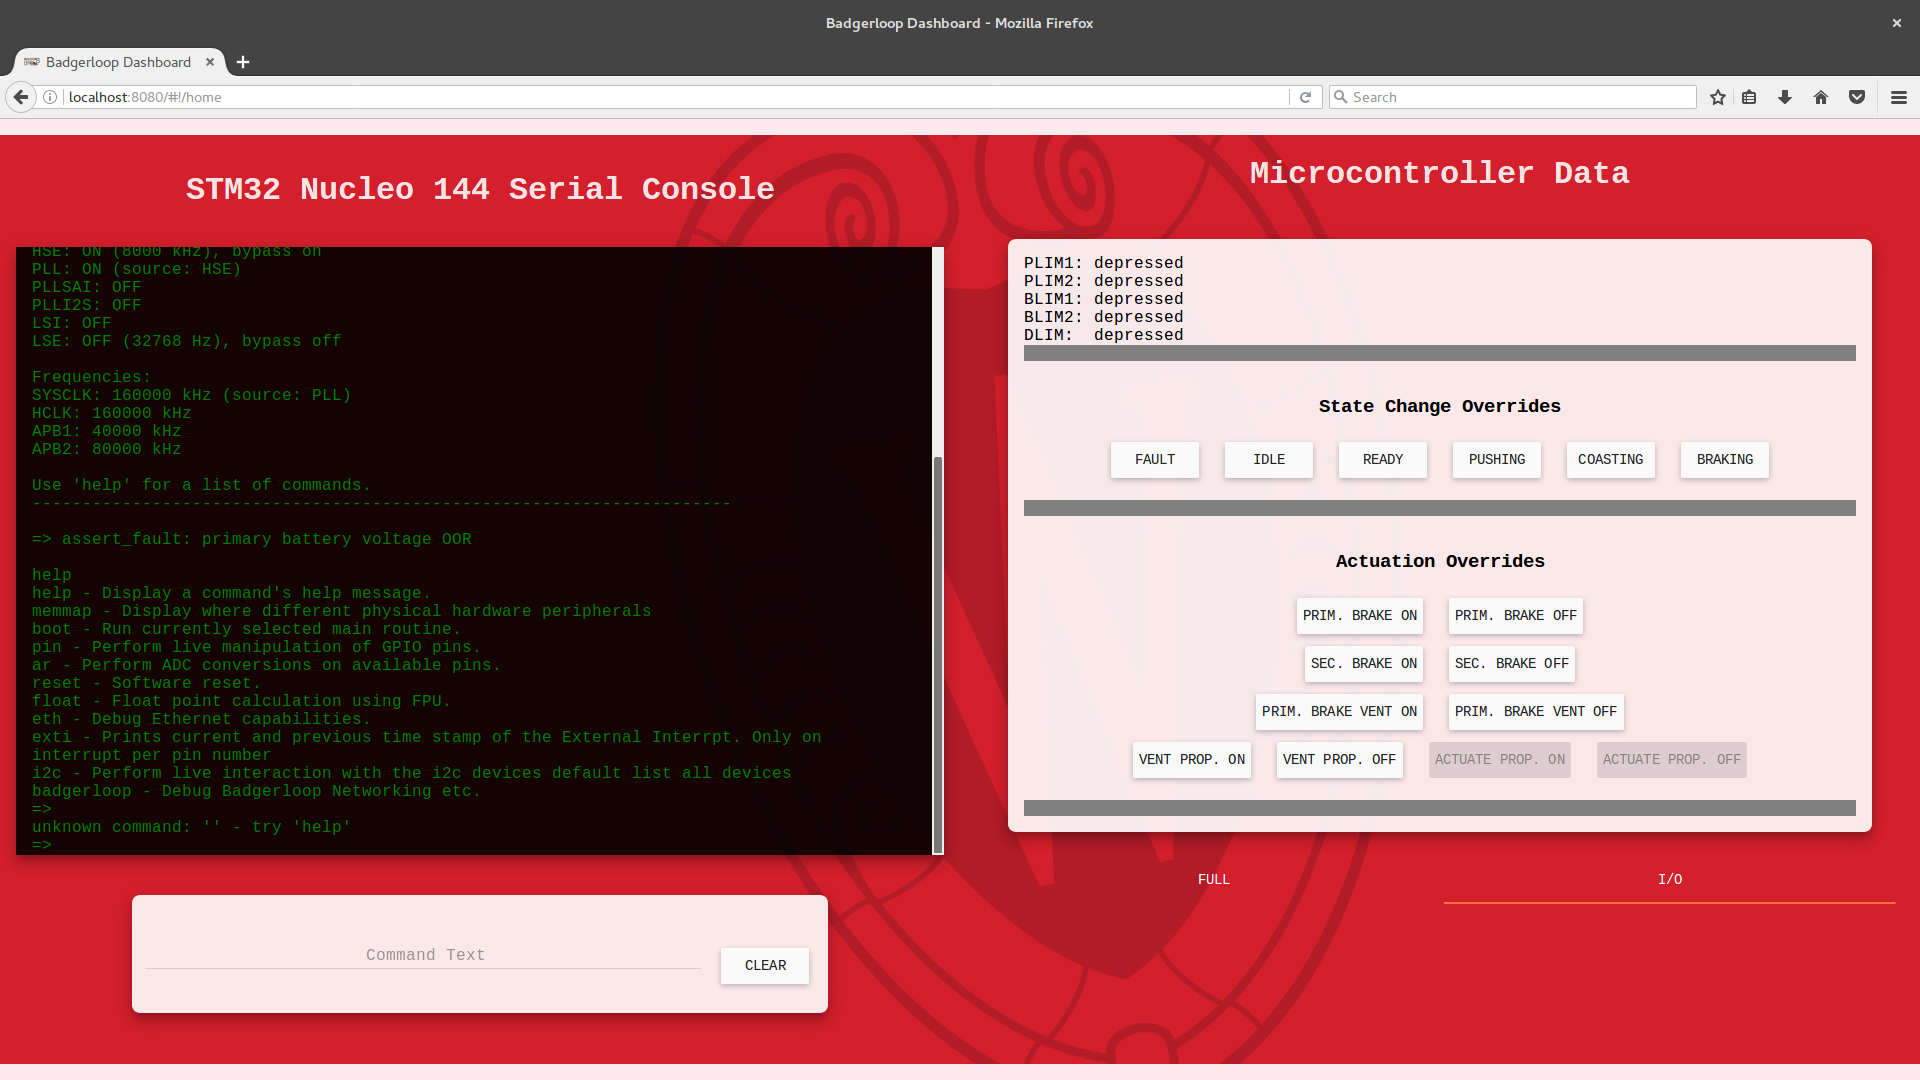
\includegraphics[width=\linewidth]{assets/badgerloop_2/Dashboard/dash_live2}
\end{center}
\end{frame}

% slide
\begin{frame}
\frametitle{Badgerloop II: Dashboard}
    \texttt{memmap} output and \texttt{badgerloop} sub-commands
\begin{center}
    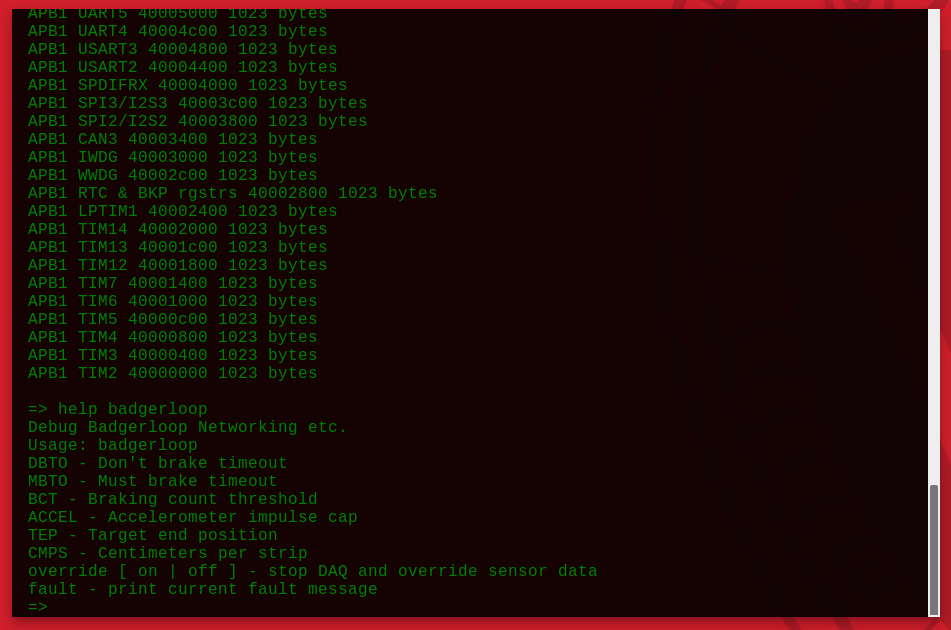
\includegraphics[width=\linewidth]{assets/badgerloop_2/Dashboard/dash_cli_example}
\end{center}
\end{frame}

% slide
\begin{frame}
\frametitle{Badgerloop II: Dashboard}
    \texttt{ar} (analog read) command output, raw 10-bit ADC
\begin{center}
    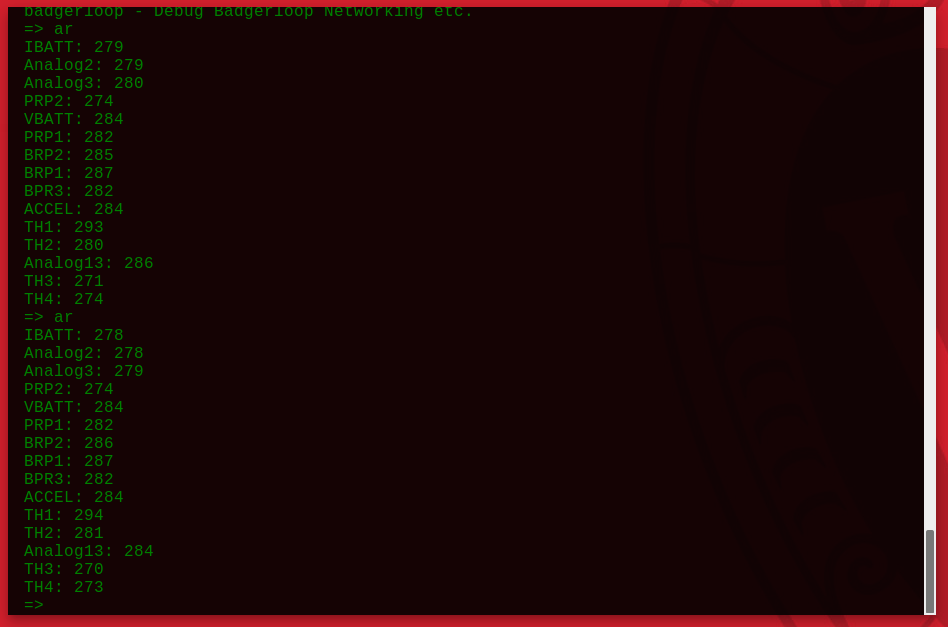
\includegraphics[width=\linewidth]{assets/badgerloop_2/Dashboard/dash_live_ar}
\end{center}
\end{frame}

% slide
\begin{frame}
\frametitle{Badgerloop II: Dashboard}
    Development on the Dashboard on the road to the competition from Wisconsin
\begin{center}
    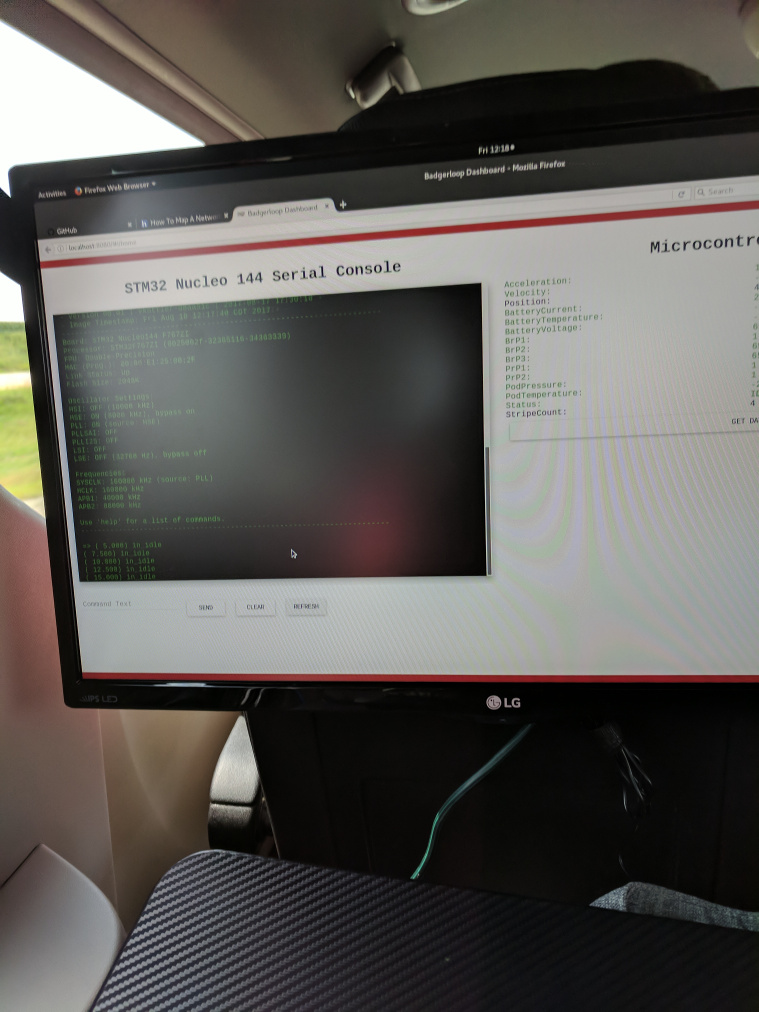
\includegraphics[height=2.5in]{assets/badgerloop_2/Dashboard/in_the_car}
\end{center}
\end{frame}

\end{document}
